\documentclass[letterpaper,spanish,11pt]{article}
\usepackage[latin1]{inputenc}    % Agregar y acentos
\usepackage{babel}               % Soporte multilenguajes
%\usepackage{avant}               % Tipo de fuente
%\usepackage{fancyheadings}       %% Topes y pies de p�ina
%\usepackage[dvips]{graphicx}     % Inclusion de imagenes .eps
\usepackage{amsmath,amsthm,url}
%\usepackage{url}                 % Agregar Links soporte de ~
\usepackage{verbatim}
%\usepackage{geometry}
\usepackage{color}
\usepackage{amsfonts}
\usepackage{amssymb}
%\usepackage{txfonts}
%\usepackage{pxfonts}
%\usepackage{fancybox}
\usepackage{latexsym}
%\usepackage{fancyvrb}
\usepackage{graphicx}
%\usepackage{pstricks}
\usepackage{setspace} % paquete para interlineado
\usepackage{url}
\usepackage{colortbl}
\usepackage{multirow}
\usepackage{slashbox}
\usepackage{rotating}
\definecolor{rojo}{rgb}{1,0,0}
\oddsidemargin -0.1in
\topmargin -0.5in
\textwidth 6.7in
\textheight 8.5in

\begin{document}

\begin{titlepage}
%\begin{figure}[htbp]
\begin{center}

\includegraphics[height=3.5cm]{logo_latex}  %se coloca solo el nombre de archivo sin .extension y la imagen en formato .png
\end{center}
%\end{figure}
\vspace{1.5cm}
\begin{center}
\textbf{\Huge{Laboratorio de estad\'istica}}\\[0.2cm]
\textbf{\Huge{computacional}}\\[0.7cm]
\textbf{\huge{Informe \# 1}}\\[0.7cm]
\textbf{\huge{``Estadistica descriptiva univariada y bivariada''}}\\[0.3cm] % en caso de que el titulo del tema sea corto, ajustar las medias para que los nombres de los integrantes queden mas abajo
\today\\[1.5cm]
\end{center}
\begin{flushright}
\large{\textbf{Profesor de C\'atedra}} \\
\large{Ricardo \~{N}anculef} \\[0.5cm]
\large{\textbf{Ayudantes de laboratorio}}\\
\large{Milciades Reyes}\\
\large{Fernando Herrera}\\[0.5cm]

\large{\textbf{Integrantes}} \\
\large{Esteban Bombal 2673004-k} \\
\large{Rodrigo Fernandez 2673002-3} \\
\large{Cristian Maureira 2673030-9} \\
\large{Gabriel Zamora 2673070-8} \\
\end{flushright}
\end{titlepage}

\section*{Descripci\'on del Fen\'omeno y del Muestreo}

\begin{enumerate}
\item Hip\'otesis: La edad de iniciaci\'on en las relaciones sexuales disminuye al aumentar el consumo de los medios de comunicaci\'on.
\item Variables a medir: Edad de iniciaci\'on sexual (entre 13 y 21 a\~nos), horas de consumo de medios de comunicaci\'on promedio al d\'ia (entre 0 y 8), categoria de la informaci\'on m\'as captada al d\'ia (Adultos, Juveniles, Telenovelas, Ayuda, Deportivos, Entretenci\'on, Culturales).
\item Metodolog\'ia de muestreo:
	\begin{enumerate}
		\item Poblaci\'on Objetivo:
				Los j\'ovenes de Chile
		\item Muestra:
				J\'ovenes de la V Regi\'on
		\item Marco Muestral:
				J\'ovenes estudiantes de diferentes colegios y universidades de la V Regi\'on. Los colegios fueron: Instituto del Puerto (San Antonio), Seminario San Rafael (Vi\~na del Mar), Jos\'e Cortes Brown (Vi\~na del Mar), Los Reyes (El Belloto), Escuela Industrial Superior (Valparaiso). Las Universidades fueron: Universidad de Vi\~na del Mar (UVM), Pontificie Universidad Cat\'olica de Valparaiso (PUCV).
		\item Metodolog\'ia utilizada:
				No-Aleatorizado y por conveniencia.
		\item Justifiaci\'on del porque elegimos esta metodolog\'ia:
       				Principalmente, fue por el gasto en tiempo que significaba el realizar una encuesta de otro tipo.\\
				Tambien encontramos que, subjetivamente, las distintas personas encuestadas que logramos contactar fueron lo suficientemente variadas como para representar una porci\'on considerable de la poblaci\'on.
	\end{enumerate}
\item Recolleci\'on de Datos:\\
	En el archivo data-inf1-*.xls se encuentran los resultados de la encuesta.

\end{enumerate}

\section*{An\'alisis Univariado}
Variable cuantitativa seleccionada: horas de consumo de medios de comunicaci\'on promedio al d\'ia\\
Criterio de clases: Criterio Binomial.

\begin{displaymath}
k = \lfloor log_2 (n) + 1\rfloor = \lfloor log_2(100) + 1 \rfloor = 7
\end{displaymath}

\begin{displaymath}
R = Dato_{max} - Dato_{min} = 8 - 0 = 8
\end{displaymath}

\begin{displaymath}
A = \frac{R + 1}{k} = \frac{8 + 1}{7} = \frac{9}{7} \approx 1.3
\end{displaymath}
Marca de clase: Por medio de la media.

\begin{enumerate}
   \item Tabla de frecuencias:\\ \\
     \begin{tabular}{ | c | c | c | c | c | c | }
        \hline
        N clase & limites de clase & marca de clase & fr absoluta & fr relativa & fr relativa acumulada \\
        \hline	
          1 & (-0.5, 0.8] & 0.15 & 13 & 0.13 & 0.13 \\
          2 & (0.8, 2.1] & 1.45 & 26 & 0.26 & 0.39 \\
          3 & (2.1, 3.4] & 2.75 & 14 & 0.14 & 0.53 \\
          4 & (3.4, 4.7] & 4.05 & 6 & 0.06 & 0.59 \\
          5 & (4.7, 6.0] & 5.35 & 24 & 0.24 & 0.83 \\
          6 & (6.0, 7.3] & 6.65 & 12 & 0.12 & 0.95 \\
          7 & (7.3, 8.6] & 7.95 & 5 & 0.05 & 1 \\
        \hline
     \end{tabular}
    \item Histograma
      \begin{figure}[htbp]
      	  \centering
  	  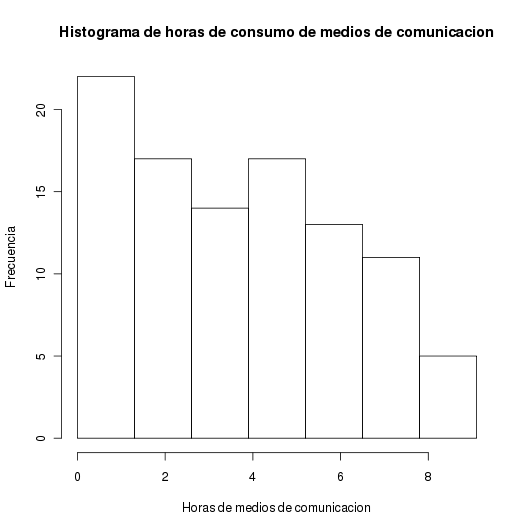
\includegraphics[width=3.3in,height=3.3in]{histograma1}
	  \caption{Histograma de frecuencias de horas de consumo de medios de comunicaci\'on}
	  \label{fig:histograma1}
      \end{figure}
    \item Medidas Agrupadas
	\begin{itemize}
		\item Media Agrupada: \\ \\
		 	$\sum_{i=1} ^n (fr_i * mc_i) = 3.709596$ \\
		\item Varianza Agrupada: \\ \\
			$\sum_{i=1} ^n (fr_i * (mc_i - media)^2) = 5.814731$ \\
		\item Desviaci\'on media Agrupada: \\ \\
			$\sqrt{\sum_{i=1} ^n (fr_i * (mc_i - media)^2)} = 2.411375$ \\
		\item Cuartiles Agrupados: \\ \\
			\begin{tabular}{|l|c|c|c|c|c|}
			\hline
			Cuartil & 1 (25\%) & 2 (50\%) & 3 (75\%) & 4 (100\%) \\
			\hline
			Rango de N\'um. de clases & [1,2) & [2,3) & [3,5) & [5,7] \\
			\hline
			Rango de valores & [-0.5,0.8) & [0.8,2.1) & [2.1,4.7) & [4.7,8.6] \\
			\hline
			\end{tabular} \\
	\end{itemize}
    \item Medidas de Tendencia
	\begin{itemize}
		\item Medidas de tendencia Central: \\ \\
			Media: $\overline{x} = \frac{\sum_{i=1} ^n x_i}{n} = 3.626263$ \\ \\
			Mediana: 3 \\ \\
			Moda: 2 (17)\\ \\
		\item Medidas de dispersi\'on: \\ \\
			\'Indice de Variaci\'on: $\ T = 1 - F_m = 1 - 0.17 = 0.83 $ \\ \\
			Varianza Muestral: $\ s^2 = \frac{1}{n} \sum_{i=1} ^n (x_i - \overline{x})^2 = 6.105538185 $ \\ \\
			Desviaci\'on Estandar: $\ s = \sqrt{\frac{1}{n}\sum_{i=1} ^n (x_i - \overline{x})^2} = 2.470938725 $ \\ \\
			Desviaci\'on Media: $\ MD = \frac{1}{n} \sum_{i=1} ^n |x_i - \overline{x}| = 2.17757578 $ \\ \\

		\item Medidas de Localizaci\'on: \\ \\
			Cuartiles: \\ \\
			\begin{tabular}{|l|c|c|c|c|c|}
			\hline
			Cuartil & 1 (25\%) & 2 (50\%) & 3 (75\%) & 4 (100\%) \\
			\hline
			Rango de valores & [0,2) & [2,3) & [3,6) & [6,8] \\
			\hline
			\end{tabular} \\
		\item Medidas de Forma (no agrupado): \\ \\
			Coeficiente de Asimetr\'ia: $\frac{\sum_{i=1}^n (x_i - \overline{x})^3}{ns^3} = 0.1229182$ \\ \\
			Coeficiente de Apuntamiento: $\frac{\sum_{i=1}^n (x_i - \overline{x})^4}{ns^4}  = 1.757481$ \\
	\end{itemize}
    \item Datos Agrupados v/s Datos No Agrupados\\\\
		\begin{tabular}{|l|c|c|}
			\hline
			& Datos Agrupados & Datos No Agrupados\\
			\hline
			Media & 3,709596 & 3.626263 \\
			\hline
			Varianza & 5,814731 & 6,105538 \\
			\hline
			Desviaci\'on Media & 2,411375 & 2,177575 \\
			\hline
			\end{tabular} \\ \\
			\\ Conclusi\'on: Por la poca diferencia entre los datos Agrupados y los No Agrupados, podemos concluir que
			 existen bastante homogeneidad entre los grupos formados, no habiendo mayor fluctuaci\'on de frecuencia entre ellos.
    \item Diagrama
	\begin{figure}[htbp]
	\centering
	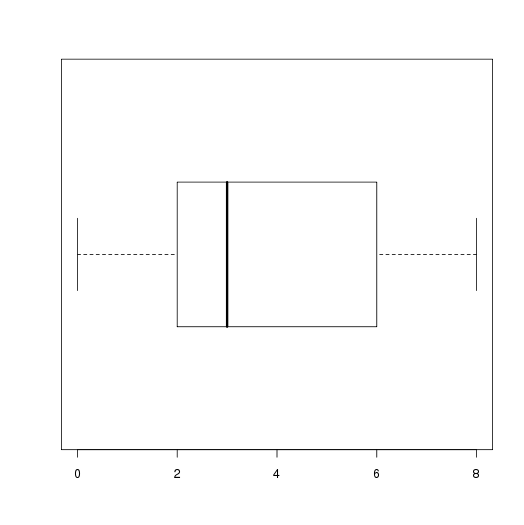
\includegraphics[width=3.3in,height=3.3in]{caja1}
	\caption{Diagrama de caja de horas de consumo de medios de comunicaci\'on}
	\label{fig:caja1}
	\end{figure}
		\begin{itemize}
		 \item Dispersi\'on de los datos:
		Los datos se concentran en mayor cantidad entre los quintiles 2 y 3, con una menor presencia de datos en los quintiles 1 y 4.\\
		 \item Tendencia:
		Los datos presentan una tendencia al valor 3, de lo cual se infiere que gracias a la mediana, se puede apreciar una mayor frecuencia de los datos que rodean este valor.\\
		 \item Existencia de \textit{outliers}:
		No existen valores fuera de los limites establecidos como buenos, concluyendo que pese a la peque\~na tendencia hacia una mediana
		 que no representa la media de los datos, se puede apreciar una homogeneidad bastante alta.
		\end{itemize}

    \item Conclusi\'on comportamiento de Datos(tomando en cuenta tambi\'en homogeneidad de los datos)\\
	\begin{itemize}
		\item En cuanto a los valores obtenidos, podemos decir que no hubieron outliers, por lo que no se presentaron datos an\'omalos con los que lidiar.
		\item Seg\'un el histograma de la secci\'on dos, podemos darnos cuenta que la cantidad de j\'ovenes va decreciendo a medida que aumentan las horas
			que le dedican a los medios de comunicaci\'on, atribuimos esto por la carga acad\'emica que presentan en el colegio y universidad.
		\item Las medidas de tendencia de las variables est\'an en un rango centrado en 3, con una desviaci\'on est\'andar cercana a 1
		\item La desviacion estandar indica un rango alrededor de la media, en la cual se encuentra la totalidad de los valores, por lo cual podemos decir
			 que debido a que es un rango peque\~no, la media predice de buena manera la totalidad de los valores
		\item Como nos dimos cuenta en el item 5, al considerar la relaci\'on entre los datos agrupados y los no agrupados, nos damos cuenta que los datos se
			 comportan de una forma homog\'enea
		\item Los datos se comportaron muy parecido a la forma que hab\'iamos predicho, ya que encontramos altos \'indices en la promiscuidad con respecto a 
			programas con un contenido con temas relacionados con sexualidad, obviamente podemos concluir que como la mayor\'ia de los encuestados no se
			hab\'ia iniciado sexualmente hace muchos a\~nos, la programaci\'on que ve\'ian era la misma
	\end{itemize}	
    \item Transformaci\'on Lineal: \\ \\
	Media: \\ \\
	Te\'orico: \\ \\
	$y = mx + b$ \\
	$\Leftrightarrow \frac{\sum_{i=1}^n y_i}{n} = \frac{\sum_{i=1}^n (m x_i + b)}{n}$ \\
	$\Leftrightarrow \overline{y} = m \overline{x} + b$ \\
	$\Leftrightarrow \overline{y} = 3 * 3.626263 + 100 = 110.878789$ \\ \\
	Pr\'actico: \\ \\
	$\overline{y} = 110.8788$ \\ \\
	
	$\therefore$ La media presenta una relaci\'on lineal. \\ \\
	
	Varianza: \\ \\
	Te\'orico: \\ \\
	$y = mx + b$ \\
	$\Leftrightarrow y - \overline{y} = mx + b - \overline{y}$ \\
	$\Leftrightarrow y - \overline{y} = mx + b - (m \overline{x} + b)$ \\
	$\Leftrightarrow y - \overline{y} = m(x - \overline{x})$ \\
	$\Leftrightarrow (y - \overline{y})^2 = m^2 (x - \overline{x})^2$ \\
	$\Leftrightarrow \sum_{i=1}^n \frac{(y_i - \overline{y})^2}{n} = m^2 \sum_{i=1}^n \frac{(x_i - \overline{x})^2}{n}$ \\
	$\Leftrightarrow$ varianza(y) = $m^2$ varianza(x) \\
	$\Leftrightarrow$ varianza(y) = 9 * 6.113997 = 55.025973 \\ \\
	P\'ractico: \\ \\
	varianza(y) = 55.02597 \\
	
	$\therefore$ La varianza de y, es proporcional a la varianza de x, a trav\'es del factor $m^2$ \\ \\
    \item �`En qu\'e intervalo centrado en la media aritm\'etica se encuentra el 81\% de los datos x?(Desigualdad de tchevichev)\\ \\
	Entre la media $\pm$ k veces la desviaci\'on t\'ipica existe, como m\'inimo, el: \\ \\
	$100(1 - \frac{1}{k^2})\%$ de las observaciones. \\ \\
	Por lo que: \\ \\
	$100(1 - \frac{1}{k^2}) = 81$\\
	$\Leftrightarrow k \approx 2.29 $ \\ \\
	$\therefore$ Al menos el 81\% de los datos se ubica en:\\ \\
	media $\pm$ ks = $3.709596 \pm 5.51$\\ \\
\end{enumerate}

\section*{An\'alisis Bivariado}
\begin{itemize}
\item Analizando las edades de iniciacion sexual y su relacion con los tipos de programa que ven al dia\\\\
La variable continua que se escogi\'o como variable dependiente son las edades de iniciacion sexual\\
La variable estratificadora categ\'orica son lass categorias de informaci\'on que m\'as captan al d\'ia.
\begin{enumerate}
\item Tabla de Contingencia con frecuencias absolutas\\\\
        \begin{tabular}[c]{|c|c c c|c|}
        \hline
        $_x\diagdown ^{y}$ & 13-15 & 16-18 & 19-21 & f.marginal \\
        \hline
        Adultos & 14 & 7 & 7 & 28 \\
        Juveniles & 12 & 6 & 3 & 21 \\
        Telenovelas & 4 & 9 & 2 & 15 \\
        Ayuda & 4 & 2 & 1 & 7 \\
        Deportivos & 4 & 5 & 6 & 15 \\
        Entretencion & 4 & 2 & 1 & 7 \\
        Culturales & 3 & 3 & 1 & 7 \\
	\hline
        f.marginal & 45 & 34 & 21 & 100 \\
        \hline
        \end{tabular}

\item Tabla de Contingencia con frecuencias relativas\\\\

        \begin{tabular}[c]{|c|c c c|c|}
        \hline
        $_x\diagdown ^{y}$ & 13-15 & 16-18 & 19-21 & fr.marginal \\
        \hline
        Adultos & 0.14 & 0.07  & 0.07 & 0.28 \\
        Juveniles & 0.12 & 0.06 & 0.03 & 0.21 \\
        Telenovelas & 0.04 & 0.09 & 0.02 & 0.15 \\
        Ayuda & 0.04 & 0.02 & 0.01 & 0.7 \\
        Deportivos & 0.04 & 0.05 & 0.06 & 0.15 \\
        Entretencion & 0.04 & 0.02 & 0.01 & 0.7 \\
        Culturales & 0.03 & 0.03 & 0.01 & 0.7 \\
	\hline
        fr.marginal & 0.45 & 0.34 & 0.21 & 1 \\
        \hline
        \end{tabular}

\item An\'alisis de Homogeneidad de las distribuciones marginales\\
      \begin{figure}[htbp]
      	  \centering
  	  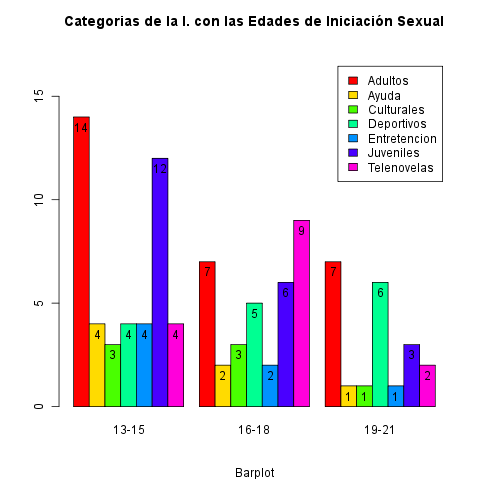
\includegraphics[width=4in,height=4in]{barplot_cat3}
	  \caption{Gr\'afico de las Categor\'ias de informaci\'on con respecto a la edad de iniciaci\'on sexual}
	  \label{fig:histograma1}
      \end{figure}\\
	Claramente, tomando en cuenta los rangos de edades de iniciaci\'on sexual, no existe algun patr\'on entre 
	las categor\'ias de la informaci\'on que obtienen de los medios de comunicaci\'on, por lo tanto \'esto nos 
	demuestra que no hay ninguna suerte de homegeneidad entre ellas.\\
	Aunque podemos ver que las categor\'ias con contenido para Adultos y Juveniles, est\'an entre las m\'as altas
	de cada rango de edad, con lo cual podemos sumar puntos a que nuestra hipotesis, se acerca a la realidad
	considerando el contenido de los programas juveniles, de hoy en d\'ia no es el m\'as adecuado para los 
	j\'ovenes  y muchas veces, se acerca mas a un contenido para adultos.\\
	Se puede observar tambi\'en que independiente de la edad en la cual se haya perdido la virginidad, la cantidad
	de personas que ven programas culturales siempre es la m\'as baja.
	En definitivas cuentas, no existe un patron por el cual las muestras se distribuyan, sino que solo es notorio
	las opciones con mas y con menos frecuencia, pero el resto se comportan de formas con respecto a la edad
	y los intereses personales de cada persona.


\item An\'alisis de dos distribuciones condicionales \\
\begin{enumerate}
\item Condicionando seg\'un las categorias de informaci\'on que m\'as captan al d\'ia\\\\
	\begin{tabular}[c]{|c|c c c|c|}
        \hline
        $_x\diagdown ^{y}$ & 13-15 & 16-18 & 19-21 & f.marginal \\
        \hline
        Adultos & 0.5 & 0.25 & 0.25 & 28 \\
        Juveniles & 0.57 & 0.29 & 0.14 & 21 \\
        Telenovelas & 0.27 & 0.6 & 0.13 & 15 \\
        Ayuda & 0.57 & 0.29 & 0.14 & 7 \\
        Deportivos & 0.27 & 0.33 & 0.4 & 15 \\
        Entretencion & 0.57 & 0.29 & 0.14 & 7 \\
        Culturales & 0.43 & 0.43 & 0.14 & 7 \\
	\hline
        \end{tabular}

\item Condicionando seg\'un la edad de iniciaci\'on sexual:\\\\
        \begin{tabular}[c]{|c|c c c|}
        \hline
        $_x\diagdown ^{y}$ & 13-15 & 16-18 & 19-21 \\
        \hline
        Adultos & 0.31 & 0.21 & 0.33 \\
        Juveniles & 0.27 & 0.18 & 0.14 \\
        Telenovelas & 0.09 & 0.26 & 0.1 \\
        Ayuda & 0.09 & 0.06 & 0.05 \\
        Deportivos & 0.09 & 0.15 & 0.29 \\
        Entretencion & 0.09 & 0.06 & 0.05 \\
        Culturales & 0.07 & 0.09  & 0.05 \\
	\hline
        f.marginal & 45 & 34 & 21 \\
        \hline
        \end{tabular}
\\\\
Analisis:
\\\\
Al parecer, a simple vista no se encuentra facilmente una relacion entre las variables. Si las agrupamos ahora en grupos ponderando el nivel de contenido sexual de cada categoria, teniendo a Adultos, Telenovelas y Juveniles con alto contenido; a Deportivos, Entretencion con moderado y a Ayuda y Culturales con bajo nivel, nos queda:\\\\

        \begin{tabular}[c]{|c|c c c|c|}
        \hline
        $_x\diagdown ^{y}$ & 13-15 & 16-18 & 19-21 & f.marginal \\
        \hline
        Alto Contenido Sexual & 30 & 22 & 12 & 64 \\
        Moderado Contenido Sexual & 8 & 7 & 7 & 22 \\
        Bajo Contenido Sexual & 7 & 5 & 2 & 14 \\
	\hline
        f.marginal & 45 & 34 & 21 & 100 \\
        \hline
        \end{tabular}
\\\\

Y si ahora vemos si analizamos sus distribuciones condicionalmente:\\

        \begin{tabular}[c]{|c|c c c|c|}
        \hline
        $_x\diagdown ^{y}$ & 13-15 & 16-18 & 19-21 & f.marginal \\
        \hline
        Alto Contenido Sexual & 0.47 & 0.34 & 0.19 & 64 \\
        Moderado Contenido Sexual & 0.36 & 0.32 &0.32 & 22 \\
        Bajo Contenido Sexual & 0.5 & 0.36 & 0.14 & 14 \\
        \hline
        \end{tabular}
\\\\

Ahora, viendo que cerca del 50\% de los jovenes que ven en los medios tem\'aticas alto contenido sexual se encuentra dentro de edades prematuras de iniciacion sexual, y tomando en cuenta que dentro de los prematuros, solo un 5\% ve contenidos de bajo contenido sexual, si podemos observar una tendencia a tener una edad prematura de iniciacion sexual mientras los medios que veas te sugeran un mayor contenido sexual.\\\\

Pero no todo es tan simple como parece. Ahora, si vemos la distribucion de los datos en base a las edades de iniciaci\'on:\\

        \begin{tabular}[c]{|c|c c c|}
        \hline
        $_x\diagdown ^{y}$ & 13-15 & 16-18 & 19-21 \\
        \hline
        Alto Contenido Sexual & 0.67 & 0.65 & 0.57 \\
        Moderado Contenido Sexual & 0.18 & 0.21 & 0.33 \\
        Bajo Contenido Sexual & 0.16 & 0.15 & 0.1 \\
	\hline
        f.marginal & 45 & 34 & 21 \\
        \hline
        \end{tabular}
\\\\

Ahora, nos podemos dar cuenta que todos los jovenes, independientemente de su edad de iniciacion secual, ven contenidos de alto, moderado y bajo contenido sexual con la misma proporcion porcentual. En vista de esto, podemos concluir que estas variables no estan relacionadas entre si de forma determinante.\\ 

\end{enumerate}
\item ?`Las Variables son independientes?\\\\
	Teniendo en Cuenta de que:\\
	\begin{itemize}
		\item \emph{X:} Categor\'as de Informac\'on
		\item \emph{Y:} Edad Iniciaci\'on Sexual
	\end{itemize}
	Adem\'as, con las tablas que obtuvimos en el item anterior, cuando se condiciono con respecto a X e Y, podemos darnos
	cuenta que no existe una independencia entre nuestras Variables.\\
		Condicionando a la variable X, en la primera fila ten\'iamos: (Cualquier fila servir\'ia como ejemplo, en \'este caso tomamos la primera)\\
		\begin{center}
			\begin{tabular}[c]{|c|c c c|c|}                           	
	                \hline
	                $_x\diagdown ^{y}$ & 13-15 & 16-18 & 19-21 \\
		        \hline
	                Adultos & 0.5 & 0.25 & 0.25 \\
			\hline
	                \end{tabular}
		\end{center}
	Claramente los valores no son iguales, ya que recordando la definici\'on para que las variables sean independientes.\\\\
	\emph{X es independiente de Y} si todas las distribuciones condicionadas $X/Y = y_{i}$ son iguales
	entre s\'i, para cualquier $y_{i}$ al que se condicione, es decir:\\
	$$f_{i/1}\ =\ f_{i/2}\ =\ f_{i/3}\ =\ f_{i/4}\ =\ \ldots$$
	En nuestro caso:
	$$0.5\ \neq\ 0.25\ \neq\ 0.25$$
	$$\therefore X\ depende\ de\ Y$$
	Perfectamente podr\'iamos llegar  a la misma conclusi\'on, si hubieramos tomado como ejemplo el \emph{condicionamiento a la variable Y}.

\item An\'alisis basado en el coeficiente de predicci\'on de Guttsman\\\\
	\textbf{Recordamos la Tabla\ de\ Contingencia}\\\\
        \begin{tabular}[c]{|c|c c c|c|}
        \hline
        $_x\diagdown ^{y}$ & 13-15 & 16-18 & 19-21 & f.marginal \\
        \hline
        Adultos & 14 & 7 & 7 & 28 \\
        Juveniles & 12 & 6 & 3 & 21 \\
        Telenovelas & 4 & 9 & 2 & 15 \\
        Ayuda & 4 & 2 & 1 & 7 \\
        Deportivos & 4 & 5 & 6 & 15 \\
        Entretencion & 4 & 2 & 1 & 7 \\
        Culturales & 3 & 3 & 1 & 7 \\
	\hline
        f.marginal & 45 & 34 & 21 & 100 \\
        \hline
        \end{tabular}\\ \\
%	Variable Predictora: Rango de edad de iniciaci\'on sexual.\\
%	Variable Dependiente: Categor\'ia de informaci\'on que consumen al d\'ia.\\ \\
	
%	$$\lambda\ = \dfrac{14+12+9+4+6+4+3-28}{100-28}\ =\ \dfrac{24}{72}\ =\ \dfrac{1}{3}$$

% En el pdf de guttmans sale que hay que hacer el mismo procedimiento, pero cambiando las variables Predictoras y Dependientes, lo hice, pero como podrán ver en los pasos siguientes, me da un lambda negativo, y no entiendo que onda :S, revisenlo para ver que onda. No pude buscar como hacer el signo lambda, porque algo raro pasa con el internet, no puedo acceder a paginas y servidores que no sean nacionales (por eso es que puedo subir cambios al git, pero, no meterme a msn, x ejemplo. Arreglo eso y sigo pendiente de esto. Saludos.

\begin{itemize}
	\item Variable Predictora: Categor\'ia de informaci\'on que consumen al d\'ia.\\
	\item Variable Dependiente: Rango de edad de iniciaci\'on sexual.\\ \\
\end{itemize}
%
%	$$\lambda\ =\ \dfrac{14+9+7-45}{100-45}\ =\ \dfrac{-15}{55}\ =\ \dfrac{-3}{11}$$
%
%	Finalmente:\\
%	$$\lambda\ =\ \dfrac{1-3}{3+11}\ =\ \dfrac{-15}{55}\ =\ \dfrac{-3}{11}$$
	
%	Para realizar el coeficiente, es mejor primero relacionar ciertas categorias entre si para simplificar un problema, y encontrar un coeficiente que explique el comportamiento general de la poblacion encuestada. Si las agrupamos ahora en grupos ponderando el nivel de contenido sexual de cada categoria, teniendo a Adultos, Telenovelas y Juveniles con alto contenido; a Deportivos, Entretencion con moderado y a Ayuda y Culturales con bajo nivel, nos queda:\\\\
	Para realizar el coeficiente, aprovechamos la clasificaci\'on realizada por categorias entre si para simplificar el problema, y encontrar un coeficiente que explique el comportamiento general de la poblacion encuestada. Por lo tanto, si las agrupamos ahora en grupos ponderando el nivel de contenido sexual de cada categoria, teniendo a Adultos, Telenovelas y Juveniles con alto contenido; a Deportivos, Entretencion con moderado y a Ayuda y Culturales con bajo nivel, nos queda:\\\\

        \begin{tabular}[c]{|c|c c c|c|}
        \hline
        $_x\diagdown ^{y}$ & 13-15 & 16-18 & 19-21 & f.marginal \\
        \hline
        Alto Contenido Sexual & 30 & 22 & 12 & 64 \\
        Moderado Contenido Sexual & 8 & 7 & 7 & 22 \\
        Bajo Contenido Sexual & 7 & 5 & 2 & 14 \\
	\hline
        f.marginal & 45 & 34 & 21 & 100 \\
        \hline
        \end{tabular}
\\\\
	Ahora para calcular el coeficiente, encontramos las frecuencias maximas de cada categoria de la variable predictora, las sumamos, y le restamos la mayor frecuencia marginal de la variable dependiente, dividido todo eso por el total de acontecimientos restandole la mayor frecuencia marginal de la variable dependiente.\\

	Con esto, nos queda:\\
	$$\lambda\ = \dfrac{(30+8+7)-45}{100-45}\ =\ \dfrac{0}{55}\ =\ 0$$\\
	
	

%
%	Para un Alto Contenido Sexual: $$22+12=34$$\\
%	Para un Moderado Contenido Sexual: $$8$$\\
%	Para un Bajo Contenido Sexual: $$7$$\\
%	
%	Total de Casos de Error: $(34+8+7)=49$\\
%
%	Por lo que nos queda:\\
%
%	$$\lambda\ = \dfrac{55-49}{55}\ =\ \dfrac{6}{55}\ =\ 0.109$$\\

%	Ahora, si vemos la relacion al reves:
%	Variable Predictoria: Rango de edad de iniciaci\'on sexual.\\
%	Variable Dependiente: Categor\'ia de informaci\'on que consumen al d\'ia.\\

%	Nos queda:\\

%	Error Original (de adivinar cuantos consumen categorias de un alto contendio sexual ):  $100-64=36$ \\
%	Error conociendo la variable ``alto contenido sexual'', suponiendo que si se iniciaron a los 13-15 a\~nos, era porque consum\'ian informaci\'on de alto contenido sexual:\\
%
%	Para 13-15 a\~nos: $30$\\
%	Para 16-18 a\~nos: $22$\\
%	Para 19-21 a\~nos: $12$\\
	
%	Total de Casos de Error: $(30+22+12)=67$\\

%	Por lo que nos queda:\\

%%	$$\lambda\ = \dfrac{36-67}{36}\ =\ \dfrac{-31}{36}\ =\ -0.86$$\\

%	\textcolor{rojo}{Como! un coeficiente negativo? revisamos la formula del coeficiente que da el libro:}


\item ?`C\'omo la variable estratificadora afecta a la variable continua?\\

	Como el coeficiente de Guttsman es cero, la variable predictora no reduce el error en la variable dependiente y su asociaci\'on entre ambas es nula.\\
	Si recurrimos al Coeficiente de Pearson tenemos que:\\ \\
	
	Tomando como:\\
	$\ x = Edades de iniciaci\'on $\\
	$\ y = Ponderaci\'on Categor\'ias de contenido$\\\\
	Calculamos:\\\\
	$\ Cov(x,y) = -0,85$\\
	$\ \sigma_x = 2,3 $\\
	$\ \sigma_y = 2,25 $ \\
	$\ \rho_x_y = -0,147$\\\\
	Entonces, teniendo un $\ \rho < 0 $, nos damos cuenta que a mayor edad de iniciación, el contenido sexual de los medios que consume es menor.\\\\ 

\end{enumerate}


\item Analizando las edades de iniciacion sexual y su relacion con la cantidad de horas dedicadas a los medios de comunicaci\'on\\\\
La variable continua que se escogi\'o como variable dependiente son las edades de iniciacion sexual\\
La variable estratificadora categ\'orica es el rango de horas dedicadas a los medios de comunicaci\'on.
\begin{enumerate}
\item Tabla de Contingencia con frecuencias absolutas\\

        \begin{tabular}[c]{|c|c c c|c|}
        \hline
        $_x\diagdown ^{y}$ & 13-15 & 16-18 & 19-21 & f.marginal \\
        \hline
        0 & 6 & 4 & 3 & 13 \\
        1 & 3 & 2 & 4 & 9 \\
        2 & 6 & 8 & 3 & 17 \\
        3 & 5 & 7 & 2 & 14 \\
        4 & 2 & 3 & 1 & 6 \\
        5 & 6 & 5 & 0 & 11 \\
        6 & 6 & 2 & 5 & 13\\
        7 & 6 & 3 & 3 & 12 \\
        8 & 5 & 0 & 0 & 5 \\
	\hline
        f.marginal & 45 & 34 & 21 & 100 \\
        \hline
        \end{tabular}


\item Tabla de Contingencia con frecuencias relativas

        \begin{tabular}[c]{|c|c c c|c|}
        \hline
        $_x\diagdown ^{y}$ & 13-15 & 16-18 & 19-21 & f.marginal \\
        \hline
        0 & 0.06 & 0.04 & 0.03 & 0.13 \\
        1 & 0.03 & 0.02 & 0.04 & 0.9 \\
        2 & 0.06 & 0.08 & 0.03 & 0.17 \\
        3 & 0.05 & 0.07 & 0.02 & 0.14 \\
        4 & 0.02 & 0.04 & 0.01 & 0.6 \\
        5 & 0.06 & 0.05 & 0 & 0.11 \\
        6 & 0.06 & 0.02 & 0.05 & 0.13\\
        7 & 0.06 & 0.03 & 0.03 & 0.12 \\
        8 & 0.05 & 0 & 0 & 5 \\
	\hline
        f.marginal & 0.45 & 0.34 & 0.21 & 100 \\
        \hline
        \end{tabular}


\item An\'alisis de Homogeneidad de las distribuciones marginales\\
      \begin{figure}[htbp]
      	  \centering
  	  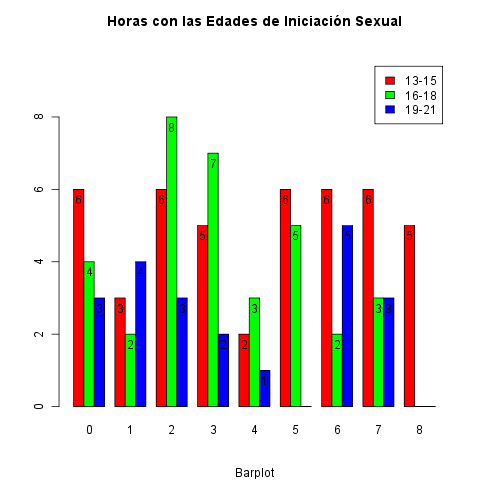
\includegraphics[width=4in,height=4in]{barplot_hor3}
	  \caption{Gr\'afico de las Horas que se le dedican a los medios con respecto a la edad de iniciaci\'on sexual}
	  \label{fig:histograma1}
      \end{figure}\\
	Ac\'a podemos observar, que los j\'ovenes que se iniciarion sexualmente entre 13-15 no poseen una cierta tendencia
	a poder obtener m\'as o menos informaci\'on de los medios de comunicaci\'on, ya que todos los valores pr\'acticamente
	se mantienen, con sus excepciones obviamente. Luego de pasar los 15 a\~nos, los j\'ovenes ya no se nutren de muchos
	medios de comunicaci\'on, quiz\'as por la responsabilidad que ya poseen, porque entre 16 y 21 a\~nos, se est\'a en la
	ense\~nanza media o en la educaci\'on superior, por eso que claramente entre 13 y 15 a\~nos, son los que m\'as se nutren
	de medios de comunicaci\'on, en \'este caso se entiende que solo es Televisi\'on, ya que es extra\~no que gente de \'esta
	edad lea diarios o escuche radio.\\
	Es dificil poder decir que nuestras frecuencias son homog\'eneas, ya que la forma como de distribuyen no presenta
	un patr\'on notorio, aparte de los se\~nalados anteriormente. 

\item An\'alisis de dos distribuciones condicionales\\
\begin{enumerate}
\item Condicionando seg\'un las horas gastadas en los medios de comunicaci\'on:\\\\
	\begin{tabular}[c]{|c|c c c|c|}
        \hline
        $_x\diagdown ^{y}$ & 13-15 & 16-18 & 19-21 & f.marginal \\
        \hline
        0 & 0.46 & 0.3 & 0.23 & 0.13 \\
        1 & 0.33 & 0.22 & 0.44 & 0.9 \\
        2 & 0.35 & 0.47 & 0.17 & 0.17 \\
        3 & 0.35 & 0.5 & 0.14 & 0.14 \\
        4 & 0.33 & 0.5 & 0.16 & 0.6 \\
        5 & 0.54 & 0.45 & 0 & 0.11 \\
        6 & 0.46 & 0.15 & 0.38 & 0.13\\
        7 & 0.5 & 0.25 & 0.25 & 0.12 \\
        8 & 1 & 0 & 0 & 0.5 \\
	\hline
        \end{tabular}

\item Condicionando seg\'un la edad de iniciaci\'on sexual:\\\\
        \begin{tabular}[c]{|c|c c c|}
        \hline
        $_x\diagdown ^{y}$ & 13-15 & 16-18 & 19-21 \\
        \hline
        0 & 0.13 & 0.12 & 0.14 \\
        1 & 0.07 & 0.06 & 0.19 \\
        2 & 0.13 & 0.24 & 0.14 \\
        3 & 0.11 & 0.21 & 0.1 \\
        4 & 0.04 & 0.12 & 0.05 \\
        5 & 0.13 & 0.15 & 0 \\
        6 & 0.13 & 0.06 & 0.24 \\
        7 & 0.13 & 0.09 & 0.14 \\
        8 & 0.11 & 0 & 0 \\
	\hline
        f.marginal & 45 & 34 & 21 \\
        \hline
        \end{tabular}
\\\\

Analisis:
\\\\
Llevando a cabo un analisis similar al usado en el primer analisis bivariado, dividimos los datos en diferentes categorias para poder analizar los datos mas facilmente:
        \begin{tabular}[c]{|c|c c c|c|}
        \hline
        $_x\diagdown ^{y}$ & 13-15 & 16-18 & 19-21 & f.marginal \\
        \hline
        0 & 6 & 4 & 3 & 13 \\
        1-2 & 9 & 10 & 7 & 26 \\
        3-4-5 & 13 & 16 & 3 & 32 \\
        6-7-8 & 17 & 5 & 8 & 30\\
	\hline
        f.marginal & 45 & 34 & 21 & 100 \\
        \hline
        \end{tabular}
\\\\
Ahora pasamos a ver las distribuciones condicionales de x e y:

         \begin{tabular}[c]{|c|c c c|c|}
        \hline
        $_x\diagdown ^{y}$ & 13-15 & 16-18 & 19-21 & f.marginal \\
        \hline
        0 & 0.46 & 0.31 & 0.23 & 13 \\
        1-2 & 0.35 & 0.38 & 0.27 & 26 \\
        3-4-5 & 0.41 & 0.50 & 0.09 & 32 \\
        6-7-8 & 0.57 & 0.17 & 0.27 & 30\\
        \hline
        \end{tabular}
\\\\
Aca podemos ver que la mayor\'ia de los que gastan mas de su tiempo en consumir informaci\'on de los medios de comunicaci\'on son los iniciados entre 13-5 a\'~nos, pero no sigue un patron linear definido con respecto al tiempo invertido por los de 16-18 y por los de 19-21. En fin, se puede intuir o pensar que los que mas tiempo invierten en los medios, son los que mas tiempo libre tienen y que terminan iniciandose sexualmente mas prec\'ozmente.\\

        \begin{tabular}[c]{|c|c c c|c|}
        \hline
        $_x\diagdown ^{y}$ & 13-15 & 16-18 & 19-21\\
        \hline
        0 & 0.13 & 0.12 & 0.14 \\
        1-2 & 0.20 & 0.29 & 0.33 \\
        3-4-5 & 0.29 & 0.47 & 0.14 \\
        6-7-8 & 0.38 & 0.15 & 0.38 \\
	\hline
        f.marginal & 45 & 34 & 21\\
        \hline
        \end{tabular}\\

Que podemos decir con respecto a los grupos de edades de iniciaci\'on sexual? Claramente se ve que la proporci\'on de gente que no invierte tiempo en los medios de comunicaci\'on, es igual para todos los estratos de edades. Despues se observa una tendencia no muy clara, en la cual parece que los iniciados sexualmente en una edad prec\'oz, consumen un poquito mas de su tiempo en los medios de comunicaci\'on. De todas formas es mejor analizar los datos a traves de los graficos y otros relaciones mas estadisticas para poder descartar/aprovar una relaci\'on entre estas variables.

\end{enumerate}

\item ?`Las Variables son independientes?\\
	Teniendo en Cuenta de que:\\
	\begin{itemize}
		\item \emph{X:} Horas gastadas en medios de comunicaci\'on
		\item \emph{Y:} Edad Iniciaci\'on Sexual
	\end{itemize}
	Podemos observar mediante las tablas de frecuencias marginales, que tanto \emph{x es dependiente de y}, como \emph{y es dependiente de x}, ya que \emph{no} se cumple que:

	$f_{i/1} = f_{i/2} = ... = f_{i/r} \ \ \ \ \forall i $\\ \\
	Esto es claro al tomar de ejemplo: \\
	
	\begin{tabular}[c]{|c|c c c|c|}                           	
	\hline
	$_x\diagdown ^{y}$ & 13-15 & 16-18 & 19-21 \\
	\hline
	0 & 0.06 & 0.04 & 0.03 \\
	\hline
	\end{tabular} \\

	$\therefore \emph{x es dependiente de y}$ \\ \\
	Por otro lado tenemos que \emph{tampoco} se cumple que:

 	$f_{1/j} = f_{2/j} = ... = f_{s/j} \ \ \ \ \forall j $\\ \\

	Esto se ve al tomar de ejemplo: \\

	\begin{tabular}[c]{|c|c|}
	\hline
	$_x\diagdown ^{y}$ & 13-15 \\
	\hline
	0 & 0.06 \\
	\hline
	1 & 0.03 \\
	\hline
	2 & 0.06 \\
	\hline
	3 & 0.05 \\
	\hline
	4 & 0.02 \\
	\hline
	5 & 0.06 \\
	\hline
	6 & 0.06 \\
	\hline
	7 & 0.06 \\
	\hline
	8 & 0.05\\
	\hline
	\end{tabular} \\

	$\therefore \emph{y es dependiente de x}$ \\ \\
\item An\'alisis basado en el coeficiente de predicci\'on de Guttsman\\

\begin{itemize}
	\item Variable Predictora: Cantidad en horas de informaci\'on de los medios de comunicaci\'on que consumen al d\'ia.\\ 
	\item Variable Dependiente: Rango de edad de iniciaci\'on sexual.\\
\end{itemize}

	Para realizar el coeficiente, aprovechamos la clasificaci\'on realizada por categorias entre si para simplificar el problema, y encontrar un coeficiente que explique el comportamiento general de la poblacion encuestada.\\\\
	
        \begin{tabular}[c]{|c|c c c|c|}
        \hline
        $_x\diagdown ^{y}$ & 13-15 & 16-18 & 19-21 & f.marginal \\
        \hline
        0 & 6 & 4 & 3 & 13 \\
        1-2 & 9 & 10 & 7 & 26 \\
        3-4-5 & 13 & 16 & 3 & 32 \\
        6-7-8 & 17 & 5 & 8 & 30\\
	\hline
        f.marginal & 45 & 34 & 21 & 100 \\
        \hline
        \end{tabular}\\\\

	Ahora, al igual que con el caso anterior, para calcular el coeficiente, encontramos las frecuencias maximas de cada categoria de la variable predictora, las sumamos, y le restamos la mayor frecuencia marginal de la variable dependiente, dividido todo eso por el total de acontecimientos restandole la mayor frecuencia marginal de la variable dependiente.\\

	Con esto, nos queda:\\
	$$\lambda\ = \dfrac{(6+10+16+17)-45}{100-45}\ =\ \dfrac{4}{55}\ =\ 0.07$$\\
	
	

%	Error Original (de adivinar el rango de edad de iniciacion sexual entre 13-15 a\~nos):  $100-45=55$ \\
%	Error conociendo la variable ``iniciacion sexual'', suponiendo que si ve entre 6-7-8 horas, se inicio a os 13-15 a�os:\\
%	Para las 0 horas: $6$\\
%	Para 1-2 horas:	$9$\\
%	Para 3-4-5 horas: $13$\\
%	Para 6-7-8 horas: $5+8=13$\\
%	
%	Total de Casos de Error: $(6+9+13+13)=41$\\
%
%	Por lo que nos queda:\\
%
%	$$\lambda\ = \dfrac{55-41}{55}\ =\ \dfrac{14}{55}\ =\ 0.25$$\\
%
%	Por lo tanto, segun el coeficiente de predicci\'on de Guttsman, las variables estan poco relacionadas entre si.
%	\\ \\
%	\textcolor{rojo}{Falta}
\item ?`C\'omo la variable estratificadora afecta a la variable continua?\\

	Como el coeficiente de Guttsman es cercano a cero, la variable predictora reduce muy poco el error en la variable dependiente (solo lo reduce un 7\%) y su asociaci\'on entre ambas es casi insignificante.\\\\

	Si recurrimos al Coeficiente de Pearson tenemos que:\\ \\
	
	Tomando como:\\
	$\ x = Cantidad de Horas que consume comunicaci\'on $\\
	$\ y = Edad de Iniciaci\'on $\\\\
	Calculamos:\\\\
	$\ Cov(x,y) = -0,88$\\
	$\ \sigma_x = 2,3 $\\
	$\ \sigma_y = 2,4 $ \\
	$\ \rho_x_y = -0,15$\\\\
	Entonces, teniendo un $\ \rho < 0 $, nos damos cuenta que a mayor edad de iniciación, la cantidad de horas que consume medios de comunicaci\'on es menor.\\\\ 

\end{enumerate}
\end{itemize}


\end{document}
